%%
%% Template conclusion.tex
%%

\chapter{User Preferences}
\label{cha:ivg}

In this chapter we will compare the predictiveness across the following different types of \emph{user preferences} available
in Facebook:
\begin{itemize}
\item \textbf{Demographics} : Age, gender and location of a user.
\item \textbf{Favourites} : A users favourite preferences for activities, books, athletes, teams, movies, music, sports, television, people and interests.
\item \textbf{Groups} : All groups a user has joined.
\item \textbf{Pages} :  All pages a user has liked.
\end{itemize}

\section{Demographics}
\label{sec:demo}

The first \emph{user preference} we will examine is \emph{demographics}, the specific \emph{demographics} data we are interested in includes:
\begin{itemize}
\item \textbf{Users age}
\item \textbf{Users birthday}
\item \textbf{Users location}
\end{itemize}

Below we will give a basic analysis of this \emph{demographics} data in our data set.

Gender breakdown:
% select count(*), lu.gender from linkrUser lu where lu.uid in (SELECT distinct uid FROM trackRecommendedLinks) group by gender;

\begin{table}[!htbp]
\centering
	\begin{tabular}{|c|c|c|} % cols: (left, center, right)
		\hline
		\textbf{Male} & \textbf{Female} & \textbf{Undisclosed}  \\ \hline
		85 & 33 & 1 \\ \hline
	\end{tabular}
	\caption{Gender breakdown for app users. We see a strong male bias.}
	\label{tab:revpol}
\end{table}

Despite this clear male bias \cite{jugand} found that in a social setting, there are no strong gender homophily tendencies. Hence the male 
skew should not negatively affect our results. Additionally \cite{backstrom2011center} have shown that different genders have differing 
tendencies to disperse interactions across genders, implying this gender bias will not negatively effect prediction and hence gender information will be used as 
part of the \emph{demographics} feature vector.

\clearpage

Birthday breakdown:

% select count(*), right(lu.birthday,4) from linkrUser lu where lu.uid in (SELECT distinct uid FROM trackRecommendedLinks) group by right(lu.birthday,4);
\begin{table}[!htbp]
\centering
	\begin{tabular}{|l|c|} % cols: (left, center, right)
		\hline
		\textbf{Year} & \textbf{Frequency}  \\ \hline
		Undisclosed & 1 \\ \hline
		1901-1905 & 1 \\ \hline
		1906-1910 & 0 \\ \hline
		1911-1915 & 1 \\ \hline
		1916-1920 & 0 \\ \hline
		1921-1925 & 0 \\ \hline
		1926-1930 & 0 \\ \hline
		1931-1935 & 0 \\ \hline
		1936-1940 & 1 \\ \hline
		1941-1945 & 0 \\ \hline
		1946-1950 & 0 \\ \hline
		1951-1955 & 0 \\ \hline
		1956-1960 & 2 \\ \hline
		1961-1965 & 1 \\ \hline
		1966-1970 & 4 \\ \hline
		1971-1975 & 10 \\ \hline
		1976-1980 & 12 \\ \hline
		1981-1985 & 25 \\ \hline
		1986-1990 & 34 \\ \hline
		1991-1995 & 25 \\ \hline
		1996-2000 & 2 \\ \hline
	\end{tabular}
	\caption{Birthday breakdown for app users. There is clearly a densely populated age range of around $18 - 30$.}
	\label{tab:revpol}
\end{table}

Birthdays are grouped in a distinct range, most users in this data set are grouped in the range of around $18 - 30$. 
\cite{jugand} have found that there is a strong effect of age on friendship preferences, which implies that many of our app users 
should share similar preferences given their age similarities and hence birthday information will be a useful component of this feature.

\clearpage

%select ll.name, count(*) from linkrUser lu join linkrLocation ll on lu.uid in (SELECT distinct uid FROM trackRecommendedLinks) and lu.location_id = ll.id group by lu.location_id;
Location breakdown:

\begin{table}[!htbp]
\centering
	\begin{tabular}{|l|c|} % cols: (left, center, right)
		\hline
		\textbf{Location} & \textbf{Frequency}  \\ \hline
		Undisclosed & 33 \\ \hline
		Ahmedabad, India & 1 \\ \hline
		Bangi, Malaysia & 1 \\ \hline
		Bathurst, New South Wales & 1 \\ \hline
		Bellevue, Washington & 1 \\ \hline
		Braddon, Australian Capital Territory, Australia & 1 \\ \hline
		Brisbane, Queensland, Australia & 2 \\ \hline
		Canberra, Australian Capital Territory & 56 \\ \hline
		Culver City, California & 1 \\ \hline
		Frederick, Maryland & 3 \\ \hline
		Geelong, Victoria & 1 \\ \hline
	\end{tabular}
	\caption{Location breakdown for app users. Most users are either undisclosed of based in Canberra where this app was developed.}
	\label{tab:revpol}
\end{table}

Given the fact that most app users are either situated in Canberra (location of the app development and deployment) or are undisclosed, 
location information will not be used by this feature vector.

For \emph{demographics} each feature vector $X$ where $X \in \mathbb{R}^I$ is composed of the cross product between the above components where:

\begin{itemize}
\item $x_1 = $ Whether the user $u$ is male, $gender_u = male$.
\item $x_2 = $ Whether the user $u$ is female, $gender_u = female$.
\item $x_3 = $ Whether the user $u$ and any user in the alters share the same gender defined by the relationship:

\[ Relationship_{u,3} = \{z | gender_u = gender_z\} \]

\item $x_4 = $ Whether the user $u$ and any user in the alters are of a different gender defined by the relationship:

\[ Relationship_{u,4} = \{z | gender_u \neq gender_z\} \]

\item $x_5 = $ Whether the user $u$ and any user in the alters set share the same birth range defined by the relationship:

\[ Relationship_{u,5} = \{z | birthrange_u = birthrange_z\} \]

\end{itemize}

In this case the functions $gender_{u}$ returns the gender of $u$ where $gender \in \{male, female\}$ and $birthrange_u$ returns 
the birthrange of $u$ where $birthrange \in \mathbb{R}$.

Applying this \emph{demographics} feature to our classifiers we obtain:

\begin{figure}[h]
	\begin{center}
		\includegraphics[scale=0.75]{results/demographics/bar_demographics.pdf}
		\caption{Accuracy results using \emph{demographics} features. \emph{Demographics} are our best performing feature so far for $k=0$ implying \emph{demographics} are predictive, 
				 however we still do not outperform our SMB baseline.}
	\end{center}
\end{figure}

The \emph{demographics} feature vector provides our best results so far for the case when $k=0$ implying \emph{demographics} are predictive, however they are still less predictive then 
our SMB baseline.

\clearpage
	
Comparing \emph{demographics} against exposure we obtain:
	
\begin{figure}[h]
	\begin{center}
		\includegraphics[scale=0.75]{results/demographics/line_demographics.pdf}
		\caption{Accuracy results for exposure using the \emph{demographics} features. As $k$ increases the predictiveness of \emph{demographics} substantially 
				 increases with it. Clearly gender and age are both predictive. Note in this case Constant = NB and LR = SVM.}
	\end{center}
\end{figure}

The exposure for \emph{demographics} shows a sizable improvement over our baselines as $k$ increases. This demonstrates that as the
number of friends who like an item increase, the predictiveness of our \emph{demographics} feature increases. 

Hence, both gender and 
age are predictive \emph{user features}.

\section{Favourites}
\label{sec:traits}

Facebook facilitates a wide variety of user selected \emph{favourites}. 
These \emph{favourites} allow a user to associate themselves with other people who share their same favourite tendencies under the below headings:

\begin{itemize}
\item \textbf{Activities}
\item \textbf{Athletes}
\item \textbf{Books}
\item \textbf{Interests}
\item \textbf{Movies}
\item \textbf{Music}
\item \textbf{People}
\item \textbf{Sports}
\item \textbf{Teams}
\item \textbf{Television}
\end{itemize}

Based on the frequency of memberships between our app users for these different \emph{favourite} categories they can be partitioned into three sets.
Below we display example tables of these three distinct frequency categories of high, medium and low: 

\begin{table}[h]
\begin{minipage}[b]{.32\textwidth}
\centering
  \begin{tabular}{|l|l|} % cols: (left, center, right)
  \hline
  	\small{\textbf{F}} & \small{\textbf{Television}} \\ \hline
		\small{20} & \small{The Big Bang [..]} \\ \hline
		\small{19} & \small{How I Met [..]} \\ \hline
		\small{14} & \small{The Simpsons} \\ \hline
		\small{13} & \small{Top Gear} \\ \hline
		\small{12} & \small{Futurama} \\ \hline
		\small{12} & \small{Scrubs} \\ \hline
		\small{11} & \small{Black Books} \\ \hline
		\small{10} & \small{Black Books} \\ \hline
		\small{10} & \small{South Park} \\ \hline
		\small{10} & \small{Family Guy} \\ \hline
		\small{9} & \small{The Daily Show} \\ \hline
		\small{8} & \small{The IT Crowd} \\ \hline
		\small{8} & \small{FRIENDS} \\ \hline
		\small{7} & \small{True Blood} \\ \hline
		\small{7} & \small{MythBusters} \\ \hline
  \end{tabular}
  \caption{\emph{Television}.}
\end{minipage}
\begin{minipage}[b]{.33\textwidth}
\centering
  \begin{tabular}{|l|l|} % cols: (left, center, right)
  \hline
  	\small{\textbf{F}} & \small{\textbf{Interest}} \\ \hline
		\small{5} & \small{Movies} \\ \hline
		\small{5} & \small{Music} \\ \hline
		\small{3} & \small{Cooking} \\ \hline
		\small{3} & \small{Sports} \\ \hline
		\small{2} & \small{Psychology} \\ \hline
		\small{2} & \small{Internet} \\ \hline
		\small{2} & \small{Video Games} \\ \hline
		\small{2} & \small{Martial arts} \\ \hline
		\small{2} & \small{Literature} \\ \hline
		\small{2} & \small{Economics} \\ \hline
		\small{2} & \small{Tennis} \\ \hline
		\small{2} & \small{Badminton} \\ \hline
		\small{2} & \small{Artificial intelligence} \\ \hline
		\small{2} & \small{Computers} \\ \hline
		\small{2} & \small{Travel} \\ \hline
  \end{tabular}
  \caption{\emph{Interests}.}
\end{minipage}
\begin{minipage}[b]{.32\textwidth}
\centering
  \begin{tabular}{|l|l|} % cols: (left, center, right)
  \hline
  		\small{\textbf{F}} & \small{\textbf{People}} \\ \hline
  		\small{2} & \small{Alan Turing} \\ \hline
		\small{1} & \small{Bender} \\ \hline
		\small{1} & \small{Maurice Moss} \\ \hline
		\small{1} & \small{Steve Jobs} \\ \hline
		\small{1} & \small{Sean Parker} \\ \hline
		\small{1} & \small{Pope Benedict XVI}\\ \hline
		\small{1} & \small{Martin Luther} \\ \hline
		\small{1} & \small{Alistair McGrath} \\ \hline
		\small{1} & \small{St Augustine} \\ \hline
		\small{1} & \small{Dennis Ritchie} \\ \hline
		\small{1} & \small{Linus Torvalds} \\ \hline
		\small{1} & \small{Richard Stallman} \\ \hline
		\small{1} & \small{C. S. Lewis} \\ \hline
		\small{1} & \small{Mike Oldfield} \\ \hline
		\small{1} & \small{Ryan Giggs} \\ \hline
  \end{tabular}
  \caption{\emph{People}.}
\end{minipage}
\end{table}

Where the first column \emph{F} displays the frequency for this \emph{favourite} and the second column denotes the type of \emph{favourite} displayed. 
Here we can see \emph{television} represents an example of a high frequency \emph{favourite}, \emph{interests} represent an example of a 
medium frequency \emph{favourite} and \emph{People} represent an example of a low frequency \emph{favourite}.
Note a full \emph{favourites} set can be found in \emph{Appendix A}.
\\ 

The different frequency levels are summarised between the \emph{favourites} associations below:
\begin{itemize}
\item \textbf{High Locality}: \emph{Music}, \emph{movies}, \emph{television} - Showing our app users appear to share similar \emph{favourites} in a media 
setting.
\item \textbf{Medium Locality}: \emph{activities}, \emph{books}, \emph{interests}, \emph{Sports} - Showing our app users share some degree of similar preferences 
across these \emph{favourites}.
\item \textbf{Low Locality}: \emph{people}, \emph{athletes}, \emph{teams} - Showing our app users do not share many similar preferences  
across these \emph{favourites} involving specific people and teams.
\end{itemize}

For \emph{favourites} each feature vector $X$ where $X \in \mathbb{R}^I$ is composed of the above components where:
\[ I = \{activities, athletes, books, interests, movies, music, people, sports, teams, television\} \]

The alters set for each $i$ is conditioned by the relationship:

\[ Relationship_{u,i} = \{z | SameMembership_{u,z,i}\} \]

In this case the $SameMembership_{u,z,i}$ function returns $True$ if a user $u$ shares a membership with user $v$ via the current \emph{favourite} $i$.

Applying this feature vector to our classifiers we obtain:

\begin{figure}[h]
	\begin{center}
		\includegraphics[scale=0.75]{results/traits/bar_traits.pdf}
		\caption{Accuracy results using the \emph{favourites} feature. \emph{Favourites} are our first feature more predictive then SMB
				 for the case when $k=0$, indicating that \emph{favourites} are highly predictive of user preferences.}
	\end{center}
\end{figure}

\clearpage

The \emph{favourites} feature shows our first improvement over our SMB baseline in both the LR and SVM case for demonstrating that 
\emph{favourites} are more predictive then any previously applied feature or method.

Comparing \emph{favourites} across our exposure we obtain:

\begin{figure}[h]
	\begin{center}
		\includegraphics[scale=0.75]{results/traits/line_traits.pdf}
		\caption{Accuracy results against exposure using the \emph{favourites} features. Clearly, \emph{favourites} are more predictive of
				 user preferences compared with our baselines and all \emph{user interactions} across all exposures $k$.}
	\end{center}
\end{figure}

This predictive trend continues with exposure where each successive increase of $k$ causes the predictiveness of our classifiers to increase
using the \emph{favourites} feature. Clearly, \emph{favourites} are highly predictive of a users like preferences.

\clearpage

Given the highly predictive nature of \emph{favourites}, we extract the model weights from the most predictive classifier of LR for the case where $k=0$.
In the following table we can see explicitly which \emph{favourites} are most predictive:

\begin{table}[h]
\begin{minipage}[b]{1.0\textwidth}
\centering
  \begin{tabular}{|l|l|l|l|} % cols: (left, center, right)
  \hline
  		\textbf{Favourite} & \textbf{Weight} & \textbf{Frequency} \\ \hline
		Activities & -5.927 $\pm$ 0.001 & 281 \\ \hline
		Television & -5.210 $\pm$ 0.0 & 1,029 \\ \hline
		Music & -3.409 $\pm$ 0.001 & 629 \\ \hline
		Movies & -2.668 $\pm$ 0.001 & 454 \\ \hline
		Interests & -1.921 $\pm$ 0.001 & 64 \\ \hline
		Sports & -1.820 $\pm$ 0.001 & 27 \\ \hline		
		Books & -1.769 $\pm$ 0.0 & 163 \\ \hline		
  \end{tabular}
  \caption{LR feature weights extracted for the case where $k=0$. The \emph{favourite} column displays the current \emph{favourite}.
  The \emph{weight} column shows the weighting given for this \emph{favourite} and the \emph{frequency} column displays the number of times 
  this \emph{favourite} was set to $1$. We find that both high and medium frequency \emph{favourites} are the most predictive.}
\end{minipage}
\end{table}

This table shows that the \emph{favourites} which exhibit a high to medium frequency have a larger influence during prediction. The most 
predictive \emph{favourites} are mostly focused on media and leisure.

\cite{brandtzag2011facebook} found that virtual interactions help reveal common interests, while real world interactions help 
support friendships. Our data supports this, these common interests or \emph{favourites} investigated above are clearly predictive 
of user likes, providing our most predictive results so far.


\section{Groups}
\label{sec:groups}

Facebook facilitates users to join \emph{groups} for a large number of different types ranging from 
local sports teams and political preferences to computer games. These \emph{groups} facilitate users to associate
themselves with other people who share a similar \emph{group} preference. We outline the most popular groups for our app users 
in the table below:

% select count(*),id,name from linkrGroups where uid in (select distinct uid from trackRecommendedLinks) group by id having count(*) > " + minSize + " and count(*) < " + maxSize + " order by count(*) desc;

\begin{table}[!htbp]
\centering
	\begin{tabular}{|l|l|} % cols: (left, center, right)
		\hline
		\textbf{\small{Frequency}} & \textbf{\small{Group Name}}  \\ \hline
		27 & \small{ANU StalkerSpace} \\ \hline
		20 & \small{Facebook Developers} \\ \hline
		15 & \small{ANU CSSA} \\ \hline
		14 & \small{CSSA} \\ \hline
		13 & \small{Australian National University} \\ \hline
		11 & \small{ANU - ML and AI Stanford Course} \\ \hline
		10 & \small{iDiscount ANU} \\ \hline
		10 & \small{Our Hero: Clem Baker-Finch} \\ \hline
		9 & \small{Students In Canberra} \\ \hline
		7 & \small{I grew up in Australia in the 90s} \\ \hline
		7 & \small{Grow up Australia - R18+ Rating for Computer Games} \\ \hline
		7 & \small{ANU Engineering Students' Association (ANUESA) 2010} \\ \hline
		7 & \small{ANU Postgraduate and Research Student Association (PARSA)} \\ \hline
		6 & \small{No, I Don't Care If I Die At 12AM, I Refuse To Pass On Your Chain Letter.} \\ \hline
		6 & \small{No Australian Internet Censorship} \\ \hline
		6 & \small{The Chaser Appreciation Society} \\ \hline
		6 & \small{Feed a Child with a Click} \\ \hline
		6 & \small{ANU Mathematics Society} \\ \hline
		6 & \small{ANU International Student Services, CRICOS Provider Number 00120C} \\ \hline
		6 & \small{2011 New \& Returning Burton \& Garran Hall} \\ \hline
		5 & \small{If You Can't Differentiate Between "Your" and "You're" You Deserve To Die} \\ \hline
		5 & \small{Keep the ANU Supermarket!!!} \\ \hline
		5 & \small{If 1m people join, girlfriend will let me turn our house into a pirate ship} \\ \hline
		5 & \small{The Great Australian Internet Blackout} \\ \hline
		5 & \small{When I was your age, Pluto was a planet.} \\ \hline
	\end{tabular}
	\caption{Popular \emph{groups} breakdown for our app users. The \emph{groups} joined by our app users exhibit a high 
			 degree of locality, many of these top rated \emph{groups} have an ANU and/or Canberra focus.}
	\label{tab:revpol}
\end{table}

\clearpage

The most popular \emph{groups} joined by our app users exhibit a high degree of ANU and/or Canberra based locality. The 
frequencies of these top \emph{groups} are consistent with the most predictive \emph{favourites} outlined in the previous section.

Given the quantity of \emph{groups} on Facebook, we need to find some optimal \emph{group} test size for our data set. 
Given memory and time constraints we tested within a range of $(100-1000)$ with an incremental step size of $100$ for each test.

The results for these tests are shown below:

\begin{figure}[h]
	\begin{center}
		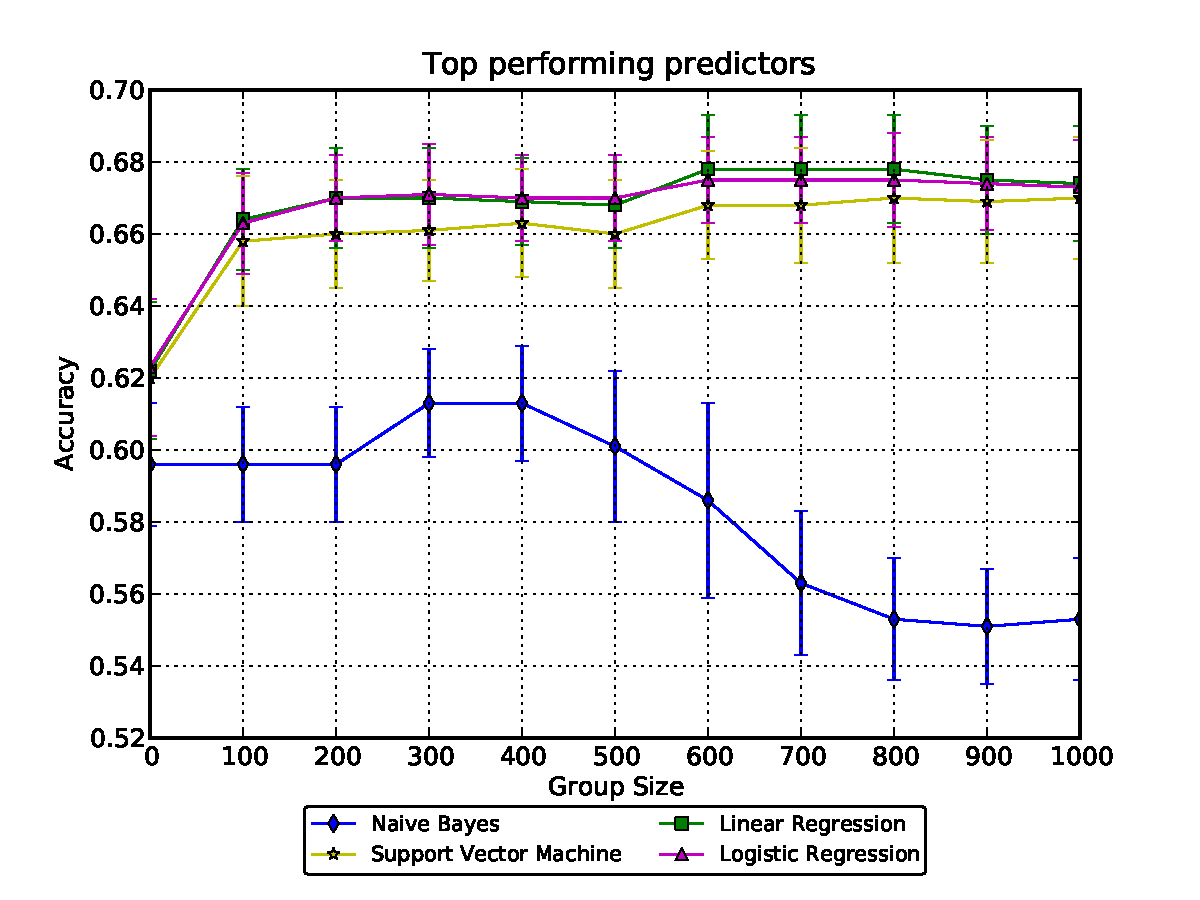
\includegraphics[scale=0.75]{results/groups/top_groups.pdf}
		\caption{Accuracy results for testing using different \emph{group} sizes. Unlike \emph{messages},
				 the predictiveness of \emph{groups} increases as the \emph{groups} size increases, implying that the more \emph{groups} considered the more 
				 predictive \emph{groups} will be.}
	\end{center}
\end{figure}

Here we see as the \emph{group} size increases, the predictiveness of this feature improves too. LR and SVM show a gradual increase 
as this \emph{group} size increases, alluding to the possibility of an even higher \emph{group} size being optimal.

The most predictive \emph{group} sizes for each of our classifiers are:
\begin{itemize}
\item \textbf{Naive Bayes}: 300
\item \textbf{Logistic Regression}: 900
\item \textbf{Support Vector Machine}: 800
\end{itemize}




For \emph{user interactions} each feature vector $X$ where $X \in \mathbb{R}^I$ is composed of the cross product between the above components where:

\[ I = \{Incoming, Outgoing\} \times \{Posts,Photos,Videos,Links\} \times \{Comments,Tags,Likes\} \]

The alters set for each $i$ is conditioned by the relationship:

\[ Relationship_{u,i} = \{z | Interacted_{u,z,i}\} \]

In this case the $Interacted_{u,z,i}$ function returns $True$ if a user $u$ has interacted with a user $v$ via the current interaction $i$.














For \emph{groups} each user $u$ and feature vector $x$ is defined as:

\[ I = \{Group\} \times \{Number of Groups\} \]

Where the optimal \emph{groups size} $J$ is defined above for each classifier.

The alters set for each $i$ is conditioned by the relationship $R$, where:

\[ R_{i,u,v} = \{z | Liked_{z,v} \wedge GroupLiked_{i,u,z}\} \]

In this case the $GroupLiked$ function returns whether both user $u$ and user $z$ have both liked the \emph{group} at index $i$.

Using the most predictive \emph{group} sizes $j$ for each of our classifiers as defined above and comparing to our baselines we obtain:

\begin{figure}[h]
	\begin{center}
		\includegraphics[scale=0.75]{results/groups/bar_groups.pdf}
		\caption{Accuracy results using the \emph{groups} feature vector. We see \emph{groups} are also more predictive over our baselines 
				 for the case where $k=0$, particularly the LR classifier.}
	\end{center}
\end{figure}

Both LR and SVM show an improvement over our SMB baseline for the case of $k = 0$ demonstrating that \emph{groups} are predictive features.

\clearpage

Applying the \emph{groups} feature against our exposure, we obtain:

\begin{figure}[h]
	\begin{center}
		\includegraphics[scale=0.75]{results/groups/line_groups.pdf}
		\caption{Accuracy results against exposure using the \emph{groups} features. Here we see that the predictive trend for the $k=0$
				 case continues with exposure for both LR and SVM.}
	\end{center}
\end{figure}

This predictive trend continues across with exposure where each successive increase of $k$ causes the performance of our LR and SVM 
classifiers to increase.

\clearpage

Given the predictive tendencies of groups, we extract the model weights for the case where $k=0$ to see which \emph{groups} 
contain the most predictive qualities:

\begin{table}[h]
\begin{minipage}[b]{1.0\textwidth}
\centering
  \begin{tabular}{|l|l|l|l|l|} % cols: (left, center, right)
  \hline
  \textbf{Name} & \textbf{Size} & \textbf{Weight} & \textbf{Frequency} \\ \hline
\small{ANU StalkerSpace} & 1292 & -7.236 $\pm$ 0 & 453 \\ \hline
\small{Facebook Developers} & 487 & -3.442 $\pm$ 0 & 177 \\ \hline
\small{ANU CSSA} & 38 & -2.742 $\pm$ 0 & 191 \\ \hline
\small{Australian National University} & 619 & -2.565 $\pm$ 0 & 70 \\ \hline
\small{Overheard at the Ateneo de Manila University} & 253 & -2.462 $\pm$ 0 & 26 \\ \hline
\small{iDiscount ANU} & 338 & -2.203 $\pm$ 0 & 88 \\ \hline
\small{PETITION FOR FACEBOOK TO INSTALL A DISLIKE BUTTON} & 683 & -2.018 $\pm$ 0 & 92 \\ \hline
\small{I grew up in Australia in the 90s} & 731 & -1.991 $\pm$ 0 & 75 \\ \hline
\small{Grow up Australia - R18+ Rating for Computer Games} & 222 & -1.951 $\pm$ 0 & 102 \\ \hline
\small{Heavy Metal - CANBERRA METAL} & 30 & -1.694 $\pm$ 0 & 42 \\ \hline
  \end{tabular}
  \caption{LR feature weights extracted for the case where $k=0$. The \emph{name} column displays the current \emph{group} name.
  The \emph{size} column shows the total size of this group across all users.
  The \emph{weight} column shows the weighting given for this \emph{group} and the \emph{frequency} column displays the number of times 
  this \emph{group} was set to $1$. We find that highly local \emph{groups} with a high frequency of app users are most predictive.}
\end{minipage}
\end{table}

\emph{Groups} are highly predictive of user preferences, we see from the weights table above that \emph{groups} which are highly local to 
the ANU and Canberra are are highly predictive as well as \emph{groups} which have a high frequency of app users.

\section{Pages}
\label{sec:pages}

Facebook facilitates users to like \emph{pages} for 'things' they like across a wide spectrum of different areas ranging from 
web browsers and TV shows to schools. This allows Facebook users to associate themselves with other users who like these similar 'things'.

\clearpage

The most popular \emph{pages} liked by our app users are shown below:

\begin{table}[!htbp]
\centering
	\begin{tabular}{|l|l|} % cols: (left, center, right)
		\hline
		\textbf{\small{Frequency}} & \textbf{\small{Page Name}}  \\ \hline
		33 & \small{ANU Computer Science Students' Association (ANU CSSA) 2011} \\ \hline
		32 & \small{The Australian National University} \\ \hline
		31 & \small{ANU Stalkerspace} \\ \hline
		21 & \small{Humans vs Zombies @ ANU} \\ \hline
		20 & \small{The Big Bang Theory} \\ \hline
		19 & \small{Australian National University} \\ \hline
		19 & \small{How I Met Your Mother} \\ \hline
		18 & \small{ANU LinkR} \\ \hline
		18 & \small{ANU ducks} \\ \hline
		17 & \small{Australian National University Students' Association} \\ \hline
		16 & \small{Google} \\ \hline
		15 & \small{Google Chrome} \\ \hline
		15 & \small{ANU XSA} \\ \hline
		15 & \small{Facebook} \\ \hline
		14 & \small{YouTube} \\ \hline
		14 & \small{The Simpsons} \\ \hline
		13 & \small{Portal} \\ \hline
		13 & \small{Top Gear} \\ \hline
		13 & \small{Music} \\ \hline
		13 & \small{ANU Memes} \\ \hline
		12 & \small{Futurama} \\ \hline
		12 & \small{Scrubs} \\ \hline
		12 & \small{ANU O-Week 2012: Escape to the East} \\ \hline
		12 & \small{The Stig} \\ \hline
		11 & \small{Black Books} \\ \hline
	\end{tabular}
	\caption{Popular \emph{pages} breakdown for our app users. \emph{Pages} exhibit less locality preferences when compared with \emph{pages},
			 while some \emph{pages} are Canberra focused, many are also more general. Additionally app user memberships for \emph{pages} is 
			 much higher then for \emph{groups}.}
	\label{tab:revpol}
\end{table}

In comparison with \emph{groups} and \emph{favourites}, \emph{pages} show a frequency across the most popular \emph{pages} for app users and 
have a less Canberra and ANU centric focus.

Given the quantity of \emph{pages} on Facebook, we need to find some optimal test size $j$ for each classifier. Given memory and time constraints we tested 
within a range of $(100-1000)$ with an incremental step size of $100$ for each test.

\clearpage

The results of these tests are shown below:

\begin{figure}[h]
	\begin{center}
		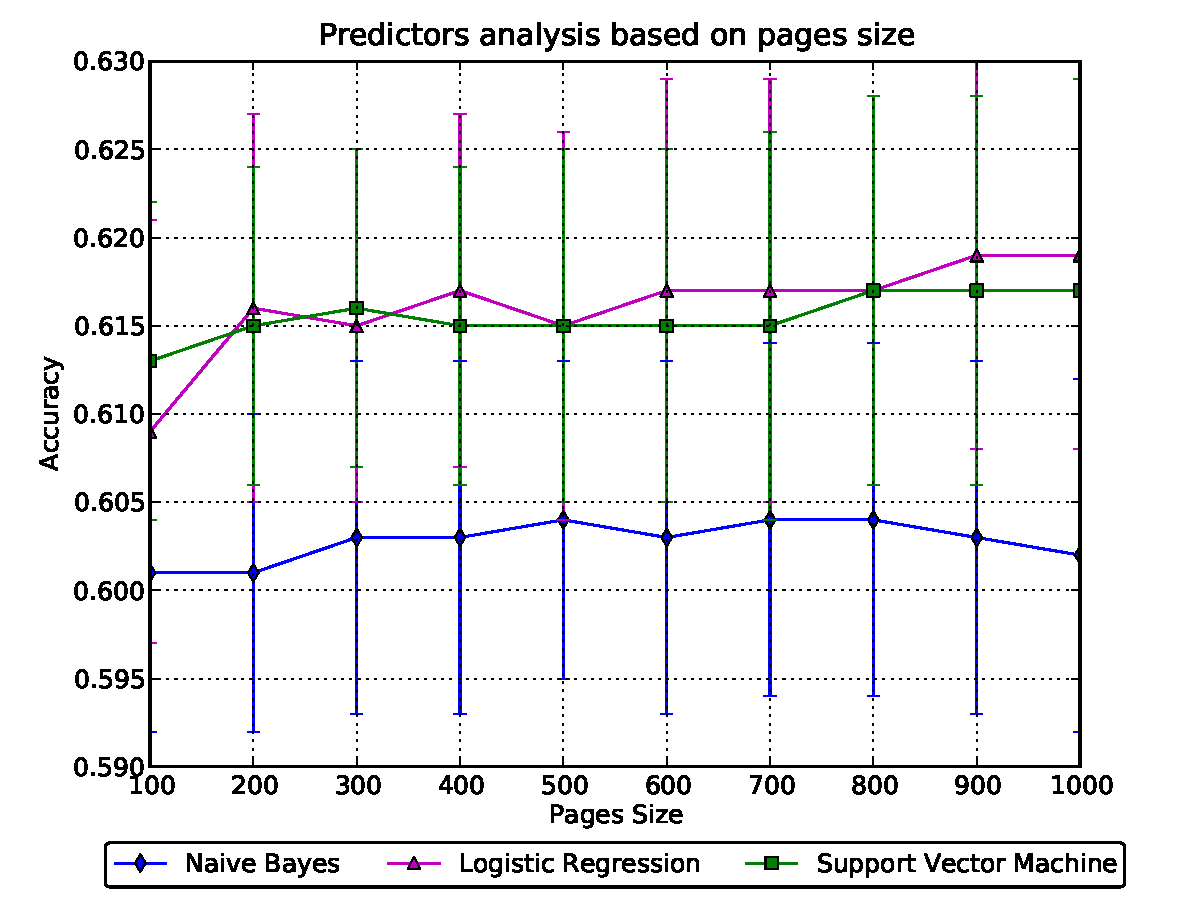
\includegraphics[scale=0.75]{results/pages/top_pages.pdf}
		\caption{Accuracy results for different \emph{page} sizes. Results for \emph{page} sizes are quite jumpy, however a similar trend 
				 from \emph{groups} follows that the more \emph{pages} we use for testing, the more predictive our results.}
	\end{center}
\end{figure}

The most predictive \emph{page} sizes $j$ for each of our classifiers are:
\begin{itemize}
\item \textbf{Naive Bayes}: 500
\item \textbf{Logistic Regression}: 900
\item \textbf{Support Vector Machine}: 800
\end{itemize}

LR and SVM exhibit a gradual increase as our \emph{page} size increases, alluding to the possibility of an even higher \emph{page}
size being optimal for prediction.

For \emph{pages} each user $u$ and feature vector $x$ is defined as:

\[ I = \{Page\} \times \{Number of Pages\} \]

Where the optimal \emph{pages size} $J$ is defined above for each classifier.

The alters set for each $i$ is conditioned by the relationship $R$, where:

\[ R_{i,u,v} = \{z | Liked_{z,v} \wedge PageLiked_{i,u,z}\} \]

In this case the $PageLiked$ function returns whether both user $u$ and user $z$ have both liked the \emph{page} at index $i$.

Using the most predictive \emph{page} sizes $j$ for each of our classifiers as defined above we obtain:

\begin{figure}[h]
	\begin{center}
		\includegraphics[scale=0.75]{results/pages/bar_pages.pdf}
		\caption{Accuracy results using the \emph{pages} feature, we can see an improvement over our baselines for both LR and SVM. 
				 Demonstrating that \emph{pages} are a predictive \emph{user preference}, however they are not as predictive as 
				 \emph{groups} or \emph{favourites}.}
	\end{center}
\end{figure}

Here we see NB, LR and SVM show an improvement over our SMB baseline for the case of $k = 0$ demonstrating that \emph{pages} are also predictive.
However, \emph{groups} and \emph{favourites} are still both more predictive. Possibly due to the fact that \emph{groups} are generally more 
local and they have a lower frequency of app user members.

\clearpage

Applying the \emph{pages} feature against exposure, we obtain:

\begin{figure}[h]
	\begin{center}
		\includegraphics[scale=0.75]{results/pages/line_pages.pdf}
		\caption{Accuracy results against exposure using the \emph{pages} feature. We see a similar trend as demonstrated in \emph{groups}
				 and \emph{favourites} where the predictiveness of this feature improves with exposure $k$.}
	\end{center}
\end{figure}

The trend of improved predictiveness over exposure $k$ continues similarly with \emph{pages}. As more data is available for the 
classifiers to learn from, their prediction accuracy increases.

\clearpage

By extracting the model weights from the case where $k=0$ we can see which \emph{pages} contain the most predictive qualities:
\begin{table}[h]
\begin{minipage}[b]{1.0\textwidth}
\centering
  \begin{tabular}{|l|l|l|l|l|} % cols: (left, center, right)
  \hline
  \textbf{Name} & \textbf{Size} & \textbf{Weight} & \textbf{Frequency} \\ \hline
\small{Sorry mate i can't, i've got Quidditch}  & 254 & -1.799 $\pm$ 0 & 18 \\ \hline
\small{Avatar: The Last Airbender}  & 324 & -1.514 $\pm$ 0.001 & 13 \\ \hline
\small{National Geographic}  & 662 & -1.437 $\pm$ 0.001 & 18 \\ \hline
\small{The Simpsons}  & 1552 & -1.414 $\pm$ 0 & 170 \\ \hline
\small{Sushi}  & 387 & -1.33 $\pm$ 0.001 & 9 \\ \hline
\small{House}  & 1746 & -1.291 $\pm$ 0 & 66 \\ \hline
\small{Seinfeld}  & 609 & -1.249 $\pm$ 0 & 15 \\ \hline
\small{Starbucks}  & 1548 & -1.249 $\pm$ 0 & 7 \\ \hline
\small{American Dad}  & 540 & -1.215 $\pm$ 0.001 & 18 \\ \hline
\small{friends don't let friends vote for Tony Abbott}  & 551 & -1.206 $\pm$ 0.001 & 19 \\ \hline
  \end{tabular}
 \caption{Negative LR feature weights extracted for the case where $k=0$. The \emph{name} column displays the current \emph{page} name.
  The \emph{size} column shows the total size of this group across all users.
  The \emph{weight} column shows the weighting given for this \emph{page} and the \emph{frequency} column displays the number of times 
  this \emph{page} was set to $1$. We find non-local and medium sized \emph{pages} to be most predictive.}
\end{minipage}
\end{table}

\begin{table}[h]
\begin{minipage}[b]{1.0\textwidth}
\centering
  \begin{tabular}{|l|l|l|l|l|} % cols: (left, center, right)
  \hline
  \textbf{Name} & \textbf{Size} & \textbf{Weight} & \textbf{Frequency} \\ \hline
\small{CatDog}  & 259 & 1.815 $\pm$ 0.001 & 12 \\ \hline
\small{Worst. Idea. Ever. [pause] Let's do it.}  & 227 & 1.737 $\pm$ 0 & 21 \\ \hline
\small{Grug}  & 279 & 1.698 $\pm$ 0 & 9 \\ \hline
\small{Kings Of Leon}  & 840 & 1.607 $\pm$ 0.001 & 14 \\ \hline
\small{Planking Australia}  & 166 & 1.598 $\pm$ 0.001 & 4 \\ \hline
\small{Dr. House}  & 964 & 1.588 $\pm$ 0 & 28 \\ \hline
\small{Suit Up}  & 466 & 1.389 $\pm$ 0.001 & 17 \\ \hline
\small{Don't you hate it when Gandalf marks your [..]}  & 110 & 1.372 $\pm$ 0.001 & 19 \\ \hline
\small{Paramore}  & 1004 & 1.343 $\pm$ 0.001 & 31 \\ \hline
\small{Tintin}  & 250 & 1.339 $\pm$ 0.001 & 11 \\ \hline
  \end{tabular}
 \caption{Positive LR feature weights extracted for the case where $k=0$. The \emph{name} column displays the current \emph{page} name.
  The \emph{size} column shows the total size of this group across all users.
  The \emph{weight} column shows the weighting given for this \emph{page} and the \emph{frequency} column displays the number of times 
  this \emph{page} was set to $1$. We find non-local and medium sized \emph{pages} to be most predictive.}
\end{minipage}
\end{table}

The most predictive \emph{pages} in our data are non-local, which was the opposite case to \emph{groups}, additionally medium sized \emph{pages}
with highly varied frequencies were the most predictive.

\section{Conclusion}
\label{sec:conc}
Throughout this chapter we have explored different \emph{user preferences} available to users to demonstrate their personal preferences across a range of 
different topics and mediums.

Others have pointed out that non-social information is more predictive of user likes \cite{www} and we observe that too.
We have found that \emph{user preferences} are more predictive of user likes compared with \emph{user interactions}, this is particularly 
true for \emph{favourites}, \emph{groups} and \emph{pages}. This observation holds true for the exposure case of $k = 0$ and our 
predictions continue to improve with each successive increase in $k$ (notably at the detriment of our baseline).

%%% Local Variables: 
%%% mode: latex
%%% TeX-master: "thesis"
%%% End: 
